\documentclass[]{book}
\usepackage{lmodern}
\usepackage{amssymb,amsmath}
\usepackage{ifxetex,ifluatex}
\usepackage{fixltx2e} % provides \textsubscript
\ifnum 0\ifxetex 1\fi\ifluatex 1\fi=0 % if pdftex
  \usepackage[T1]{fontenc}
  \usepackage[utf8]{inputenc}
\else % if luatex or xelatex
  \ifxetex
    \usepackage{mathspec}
  \else
    \usepackage{fontspec}
  \fi
  \defaultfontfeatures{Ligatures=TeX,Scale=MatchLowercase}
\fi
% use upquote if available, for straight quotes in verbatim environments
\IfFileExists{upquote.sty}{\usepackage{upquote}}{}
% use microtype if available
\IfFileExists{microtype.sty}{%
\usepackage{microtype}
\UseMicrotypeSet[protrusion]{basicmath} % disable protrusion for tt fonts
}{}
\usepackage[margin=1in]{geometry}
\usepackage{hyperref}
\hypersetup{unicode=true,
            pdftitle={Aide pour l'application CoralGrowth},
            pdfauthor={Benrezkallah Jordan},
            pdfborder={0 0 0},
            breaklinks=true}
\urlstyle{same}  % don't use monospace font for urls
\usepackage{natbib}
\bibliographystyle{apalike}
\usepackage{longtable,booktabs}
\usepackage{graphicx,grffile}
\makeatletter
\def\maxwidth{\ifdim\Gin@nat@width>\linewidth\linewidth\else\Gin@nat@width\fi}
\def\maxheight{\ifdim\Gin@nat@height>\textheight\textheight\else\Gin@nat@height\fi}
\makeatother
% Scale images if necessary, so that they will not overflow the page
% margins by default, and it is still possible to overwrite the defaults
% using explicit options in \includegraphics[width, height, ...]{}
\setkeys{Gin}{width=\maxwidth,height=\maxheight,keepaspectratio}
\IfFileExists{parskip.sty}{%
\usepackage{parskip}
}{% else
\setlength{\parindent}{0pt}
\setlength{\parskip}{6pt plus 2pt minus 1pt}
}
\setlength{\emergencystretch}{3em}  % prevent overfull lines
\providecommand{\tightlist}{%
  \setlength{\itemsep}{0pt}\setlength{\parskip}{0pt}}
\setcounter{secnumdepth}{5}
% Redefines (sub)paragraphs to behave more like sections
\ifx\paragraph\undefined\else
\let\oldparagraph\paragraph
\renewcommand{\paragraph}[1]{\oldparagraph{#1}\mbox{}}
\fi
\ifx\subparagraph\undefined\else
\let\oldsubparagraph\subparagraph
\renewcommand{\subparagraph}[1]{\oldsubparagraph{#1}\mbox{}}
\fi

%%% Use protect on footnotes to avoid problems with footnotes in titles
\let\rmarkdownfootnote\footnote%
\def\footnote{\protect\rmarkdownfootnote}

%%% Change title format to be more compact
\usepackage{titling}

% Create subtitle command for use in maketitle
\newcommand{\subtitle}[1]{
  \posttitle{
    \begin{center}\large#1\end{center}
    }
}

\setlength{\droptitle}{-2em}

  \title{Aide pour l'application `CoralGrowth'}
    \pretitle{\vspace{\droptitle}\centering\huge}
  \posttitle{\par}
    \author{Benrezkallah Jordan}
    \preauthor{\centering\large\emph}
  \postauthor{\par}
      \predate{\centering\large\emph}
  \postdate{\par}
    \date{2019-04-29}

\usepackage{booktabs}

\begin{document}
\maketitle

{
\setcounter{tocdepth}{1}
\tableofcontents
}
\chapter{Utilisateur}\label{utilisateur}

L'application \emph{Coral Growth} permet de suivre l'évolution de la
croissance de boutures de corail à partir de l'URL d'un Googlesheets.

Ce chapitre est destiné à ceux désirant de comprendre l'utilisation de
l'application. Dans le chapitre, il y aura des explications destiné à
ceux voulant comprendre le fonctionnement de l'application.

\section{Tableur Googlesheets}\label{tableur-googlesheets}

Afin de mieux comprendre comment fonctionne l'application, il est
important de connaître le jeu de donnée (dataframe).

Le tableur est divisé en 12 colonnes :

\begin{itemize}
\tightlist
\item
  project : différencie chaque expérience réalisée, généralement on
  recréera un nouveau tableur pour chacune des expériences
\item
  date : date et heure à laquelle les relevés de mesures ont été pris
\item
  author : nom de la personne ayant encodé dans le tableur
\item
  aqua : nom du mésocosme où la bouture a été prélevé
\item
  condition : condition spécifique appliquée à la bouture (exemple :
  stress hypersalin)
\item
  species : nom de l'espèce mesurée
\item
  id : numéro de la bouture mesurée
\item
  weight : masse immergée mesurée
\item
  temperature : température de l'eau de mer
\item
  salinity : salinité de l'eau de mer
\item
  status : état de santé de la bouture
\item
  comment : commentaire
\end{itemize}

\begin{figure}
\centering
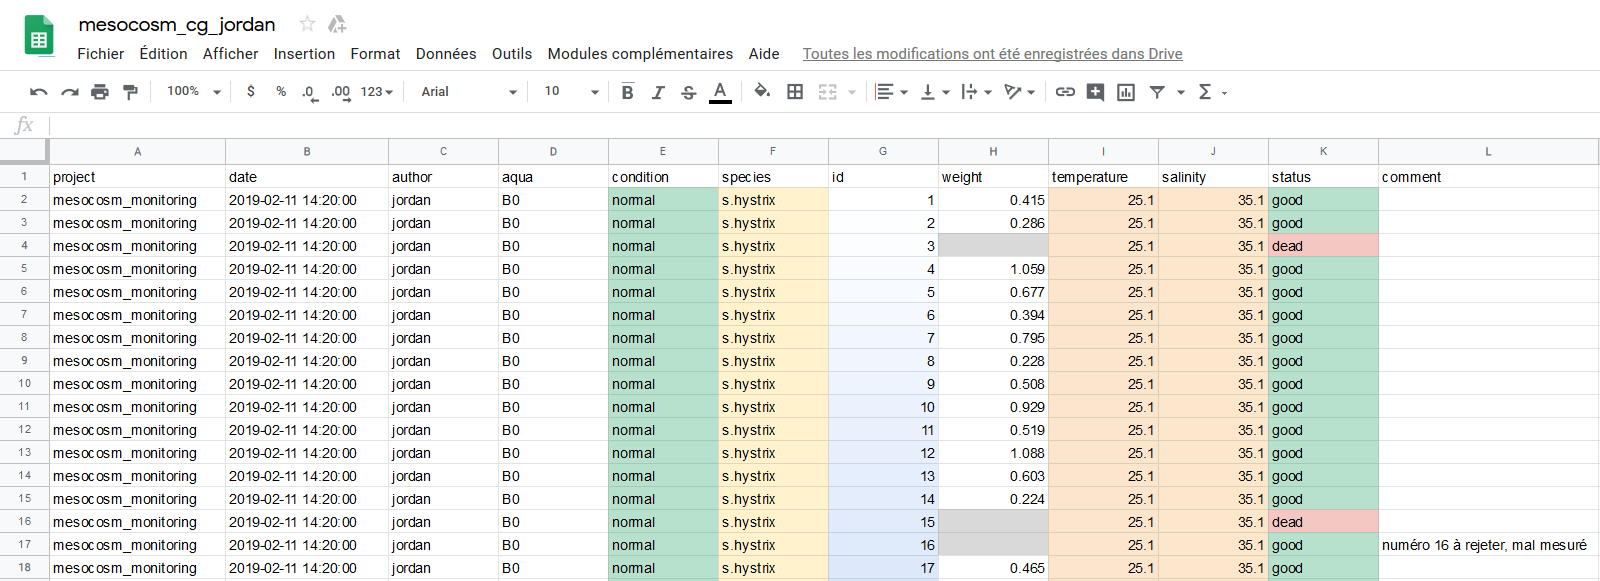
\includegraphics{image/notebook-googlesheets-presentation.png}
\caption{}
\end{figure}

\section{Onglet graphique}\label{onglet-graphique}

Le premier onglet ``Plot'', permet la visualisation sous forme de
graphique de la croissance du corail.
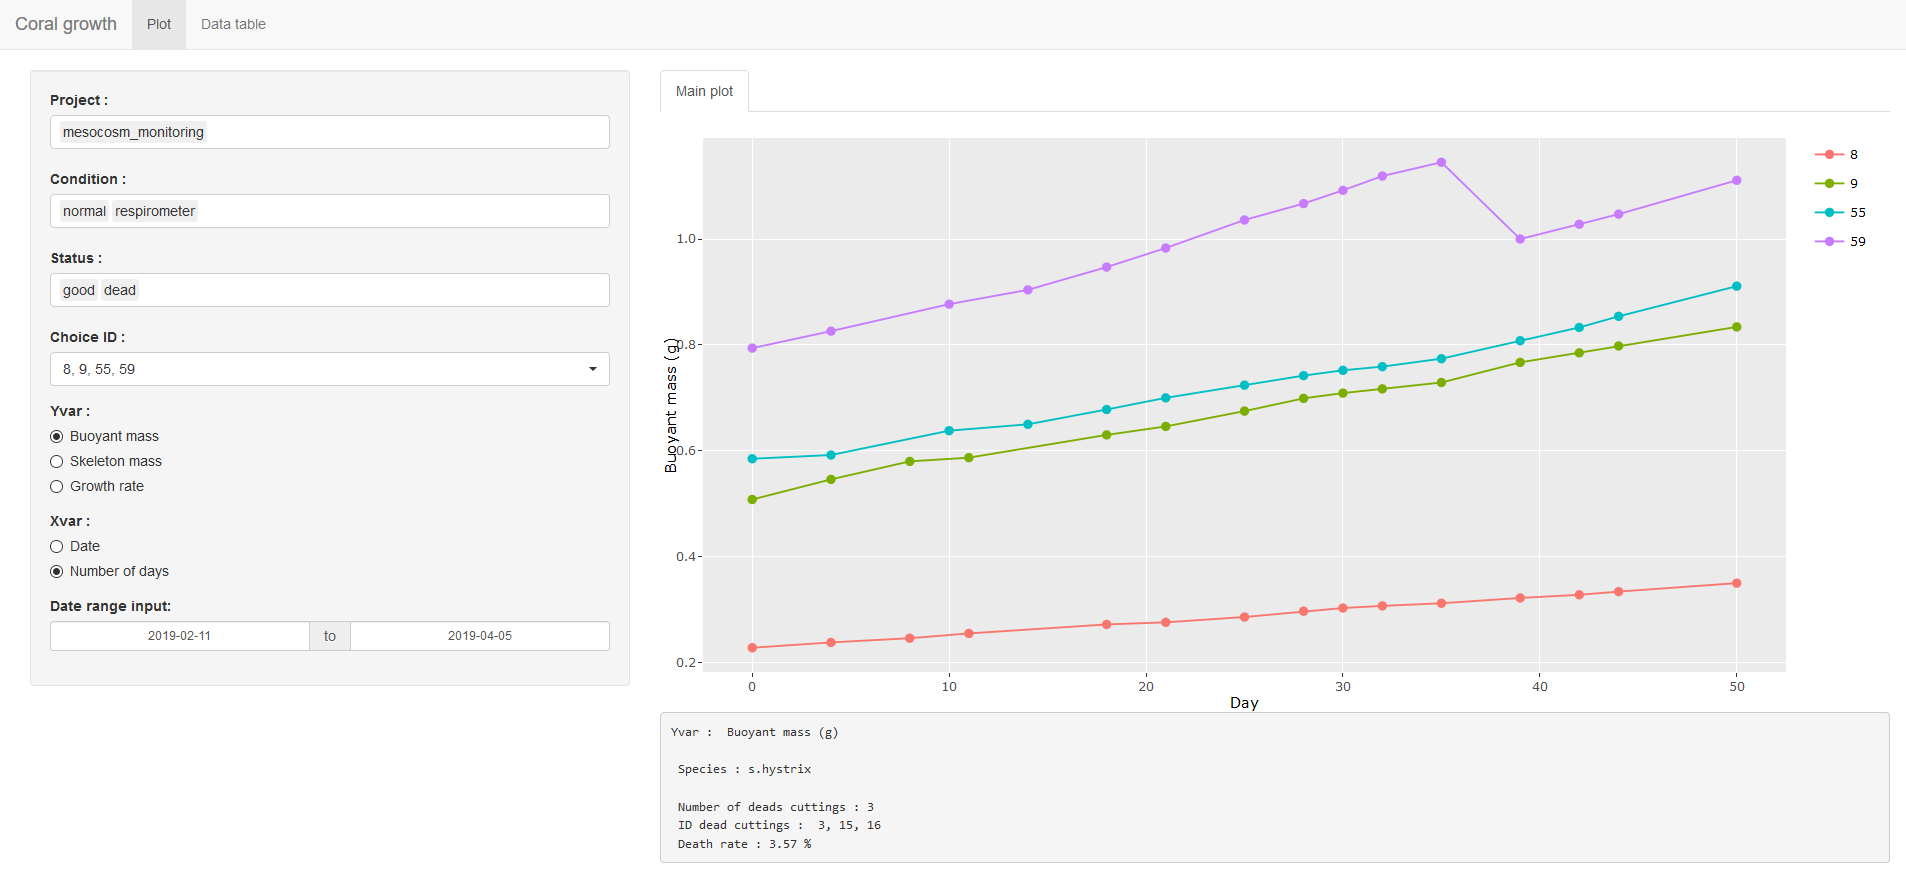
\includegraphics{image/notebook-plot1.png}

\section{Paramètres}\label{parametres}

On peut filtrer sur différents paramètres :

\begin{itemize}
\tightlist
\item
  projet
\item
  condition
\item
  statut
\item
  ID
\item
  Yvar
\item
  Xvar
\item
  période de temps
\end{itemize}

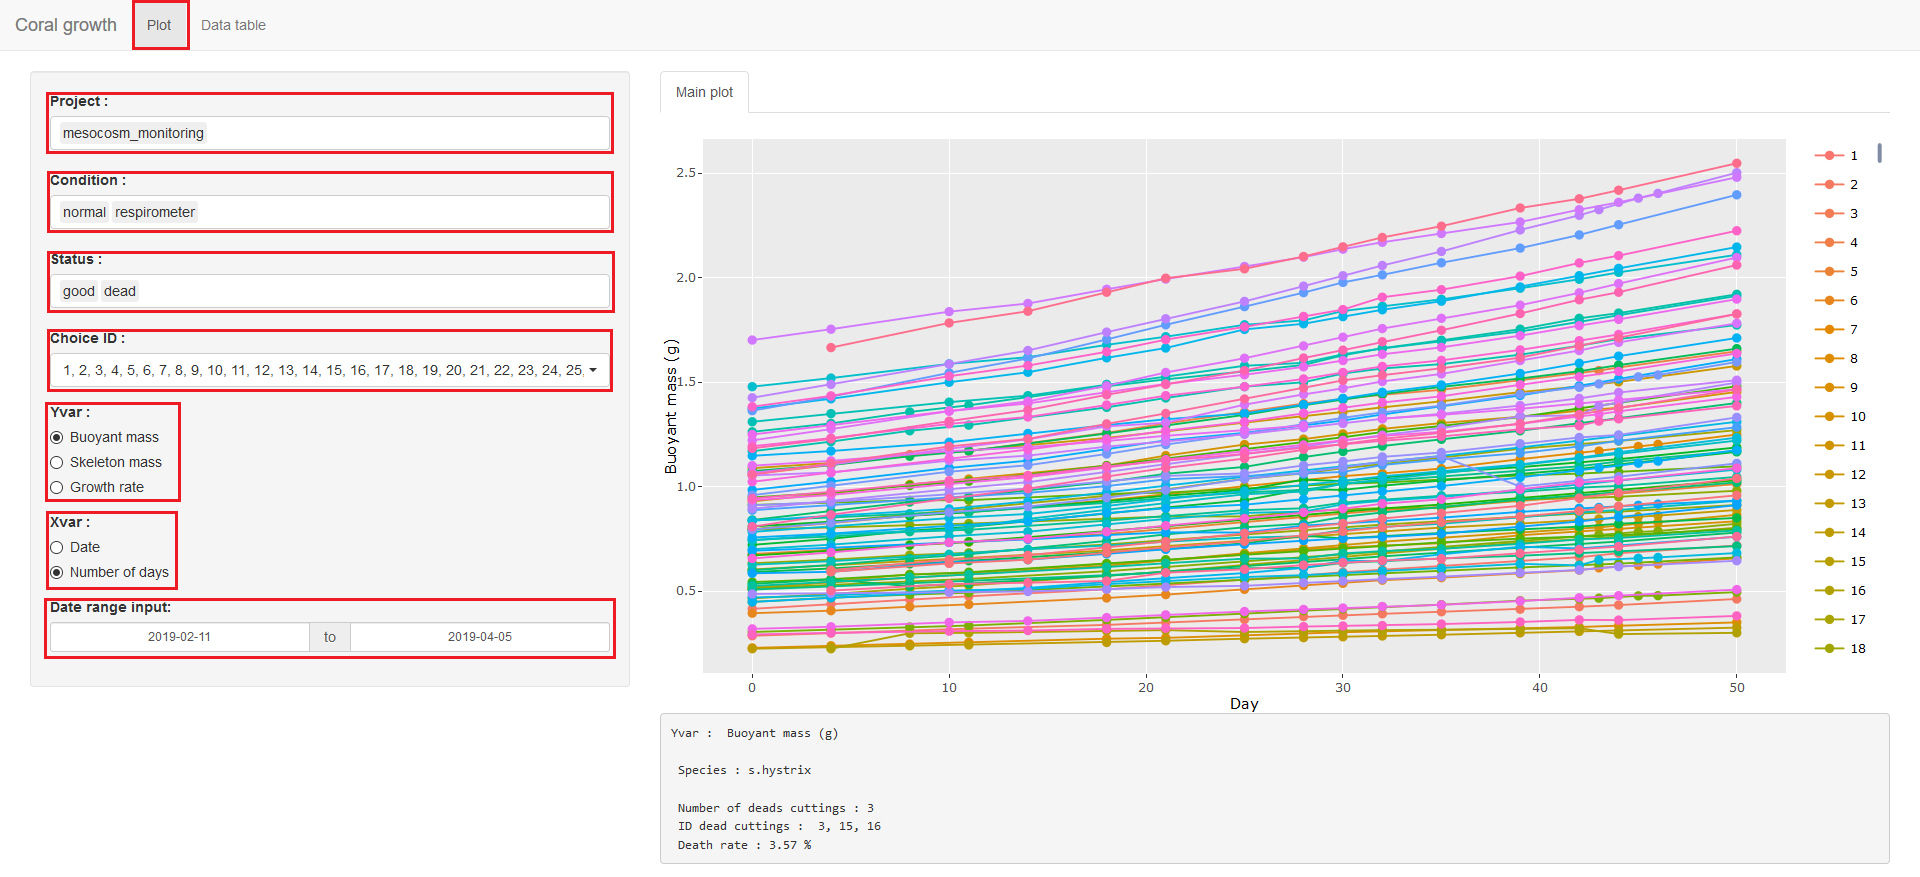
\includegraphics{image/notebook-plot2.png} Les 3 premiers paramètres
\textbf{project}, \textbf{condition}, \textbf{status} peuvent être
sélectionné depuis un menu déroulant, pour supprimer une valeur il
suffit de cliquer sur la valeur et d'appuyer sur la touche \emph{SUPPR}.

Le choix des \textbf{ID} se fait via un menu déroulant qui permet de les
sélectionner un par un ou de tout sélectionner/désélectionner.

\textbf{Yvar} permet de calculer le graphique en fonction de l'ordonnée
désirée. \emph{Buoyant mass} correspond à la masse immergée brute de la
bouture. \emph{Skeleton mass} correspond à la masse squelettique de la
bouture. Elle est calculée à partir de la masse immergée, de la salinité
et de la température à l'aide de la formule ci-dessous mise au point par
Jokiel \emph{et al} (1978) :

\begin{equation}
\large
  m_{squelettique} = \frac {m_{immerge}}{ \frac{1 - \rho_{eau}}{ \rho_{squelettique}}}
\end{equation}

\(\rho_{eau}\) est déterminé via l'équation d'état de l'eau de mer grâce
à la mesure de la salinité et de la température. Le
\(\rho_{squelettique}\) est la densité de
l'aragonite(CaCO\textsubscript{3}) du squelette du corail.

 \emph{Growth rate} correspond au taux de croissance. Elle est calculée
à partir de la masse squelettique et de la date :

\begin{equation}
\large
  Rate_{Growth} = \frac {m_{squelettique(n)}- m_{squelettique(n-1)}}{ \frac{m_{squelettique(n-1)}}{time(n) - time(n-1)}}
\end{equation}

\textbf{Xvar} permet de calculer le graphique en fonction de l'abscisse
désirée. \emph{Date} correspond à l'affichage en fonction du jour au
format \emph{MMM-dd} (exemple :Feb 15). \emph{Number of days} correspond
à l'affichage en fonction du nombre de jours écoulés depuis la première
date. Il y a un arrondi au jour près.

\textbf{Date range input} permet de sélectionner une période donnée.

\section{Graphique}\label{graphique}

En passant son curseur sur les points du graphique, on peut obtenir des
informations supplémentaires. On peut également désélectionner les
lignes en cliquant sur le numéro associer à la couleur de l'ID à droite
de l'écran.

En bas du graphique des informations supplémentaires sont données :

\begin{itemize}
\tightlist
\item
  Yvar : l'ordonnée du graphique
\item
  Species : l'espèce des boutures
\item
  Number of deads cuttings : le nombre de boutures mortes
\item
  ID dead cuttings : l'ID des boutures mortes
\item
  Death rate : le taux de mortalité
\end{itemize}

\subsection{Onglet tableau de donnée}\label{onglet-tableau-de-donnee}

Le deuxième onglet ``Data table'', permet de visualiser le tableau de
donnée, certaines colonnes ont été calculées. On peut le trier en
fonction de chacune des colonnes.
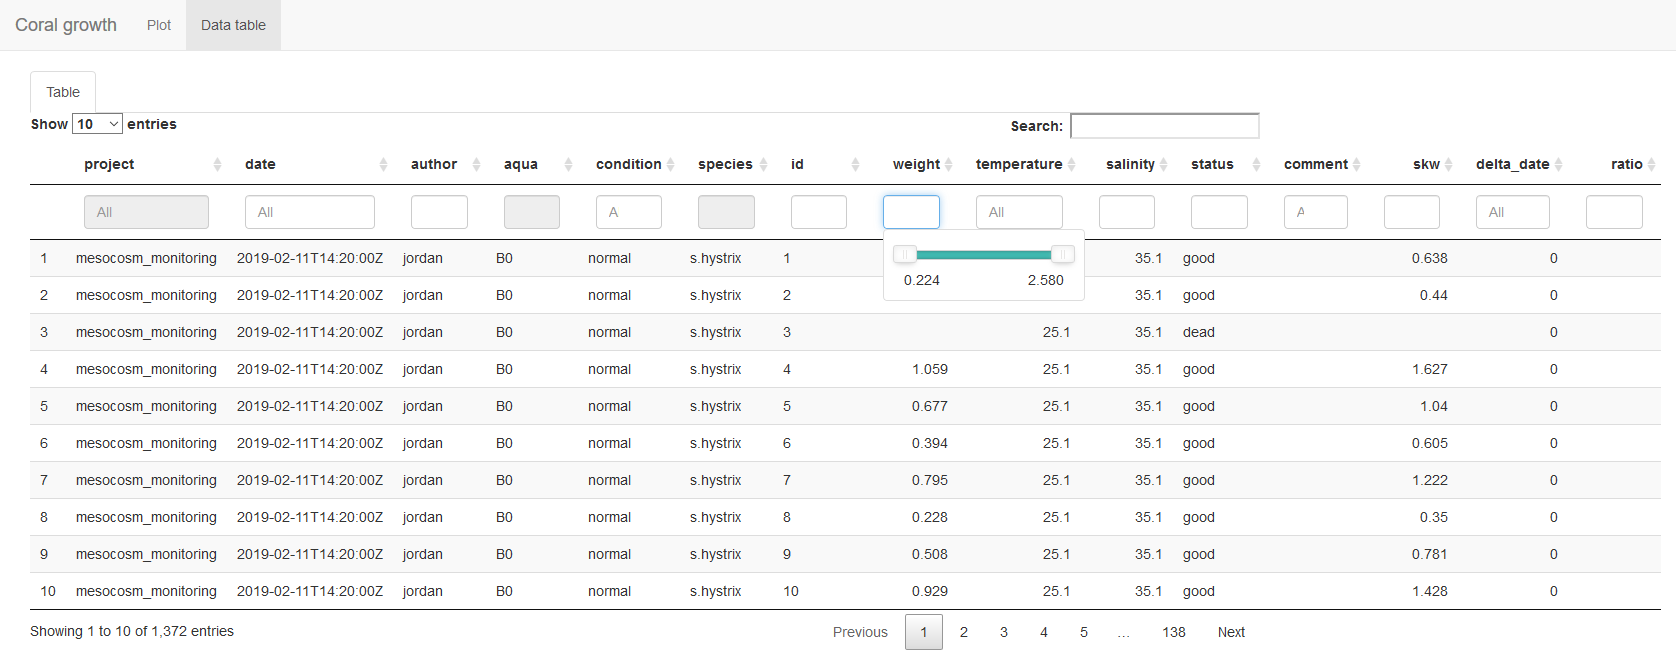
\includegraphics{image/notebook-table1.png}

\section{Accéder à l'application}\label{acceder-a-lapplication}

Il est possible d'accéder à l'application depuis cette URL :
\url{https://jack177.shinyapps.io/coralgrowth/}

Ou en scannant ce QRcode :

\begin{figure}
\centering

\includegraphics{image/QRcode.png}
\caption{}
\end{figure}

\chapter{IT}\label{it}

Ce chapitre permet de comprendre la création de l'application
\textbf{CoralGrowth}. \#\# Structure du code L'application est divisée
en deux fichiers : ui.R et server.R .

Le script ui.R contient tous les éléments à afficher à l'utilisateur. Le
script server.R contient toute la partie logique (importation du jeu de
donnée, transformation, calculs, \ldots{}) .

Les noms des variables ont un sens pratique :

\begin{itemize}
\tightlist
\item
  ui\_nom\_de\_variable : variable seulement utilisée dans le script
  ui.R .
\item
  u\_nom\_de\_variable : variable crée dans ui.R, utilisé dans server.R
  .
\item
  s\_nom\_de\_variable : variable crée dans server.R, utilisé dans
  server.R .
\end{itemize}

Les variables ``\emph{uiOutput}'' sont un peu spéciales, elles sont
crées dans ui.R, pour être configuré dans server.R . L'intérêt est d'y
insérer des variables retravaillées dans le script server.R . Ce qui
n'est pas possible si elles avaient été directement paramétrer dans ui.R
. Elles sont paramétrées dans server.R comme n'importe quelle variable
\emph{nomInput} (inputId, label, \ldots{}).

\section{server.R}\label{server.r}

\subsection{Importation}\label{importation}

L'adresse URL est contenue dans la variable coral\_url. L'URL est
générée via un fichier en ligne Google sheets.
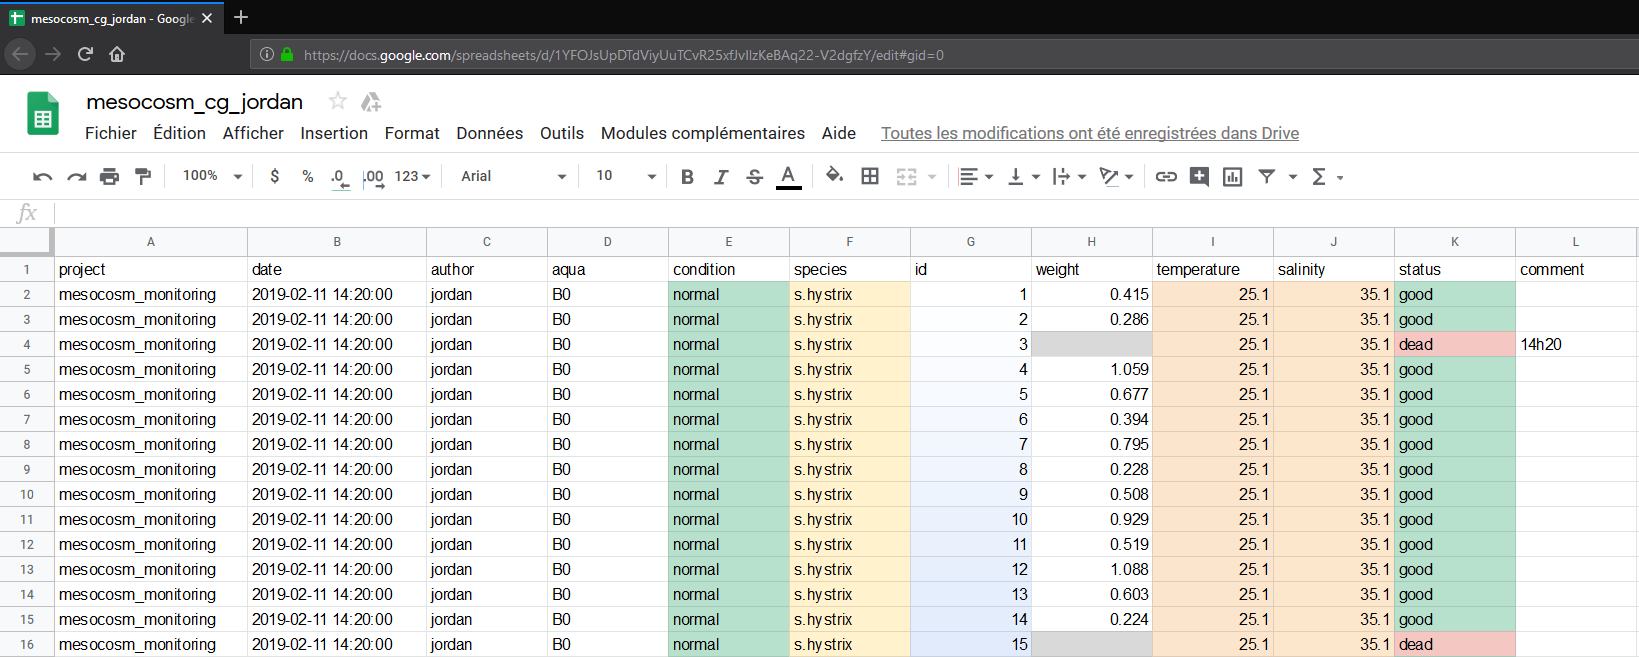
\includegraphics{image/notebook-googlesheets0.png}

Pour cela il faut aller dans \emph{Fichier \textgreater{} Publier sur le
web}, puis choisir : \emph{Intégrer \textgreater{} Valeurs séparées par
des virgules (.csv)}. 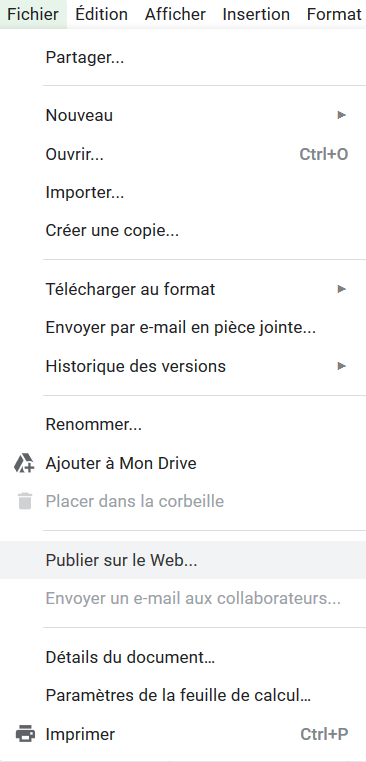
\includegraphics{image/notebook-googlesheets1.png}
\_\_\_\_\_\_\_\_\_\_\_\_\_\_\_\_\_\_\_\_\_\_\_\_\_\_\_\_\_\_\_\_\_\_\_\_\_\_\_\_\_\_\_\_\_\_\_\_\_\_\_\_\_\_\_\_\_\_\_\_\_\_\_\_\_\_\_\_\_\_\_\_\_\_\_\_\_\_\_
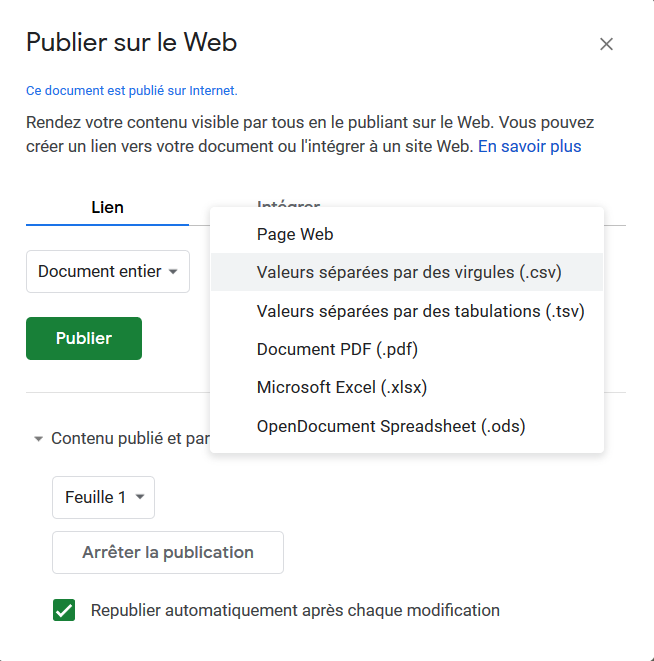
\includegraphics{image/notebook-googlesheets2.png}

Le lien de partage au format csv contenu dans \emph{coral\_url} sera lu
par la fonction \emph{read\_csv}. Cette fonction va importer le tableau
de donnée et les mettre au bon format. Une grande source d'erreur
provient de l'importation, il est important de respecter le nom des
colonnes, ne pas jouer avec le format des colonnes, surtout pour la date
qui devient facilement un problème. Dans le tableau de donnée de base,
la plupart des colonnes ont le format ``texte brute'', seuls les
colonnes ``id'', ``weight'', ``temperature'' et ``salinity'' ont un
format numérique.

\section{À notifier}\label{a-notifier}

\subsection{Colonne ratio}\label{colonne-ratio}

La colonne \emph{ratio} est calculée à partir de la première valeur
encodée de la masse squelettique avec la valeur suivante pour chacun des
ID.

Si certaines valeurs n'ont pas été rentrées lors de la première date, le
ratio ne peut être calculé.

\subsection{Colonne delta\_date}\label{colonne-delta_date}

La colonne \emph{delta\_date} est une valeur arrondie au jour près.

\subsection{Variable dateRangeInput}\label{variable-daterangeinput}

La variable \emph{dateRange} possède une plage minimum qui débute avec
la date la plus ancienne et maximum qui est la date actuelle de
l'ordinateur.

\section{À améliorer}\label{a-ameliorer}

L'application n'est pas parfaite, elle pourrait être encore plus utile.
Je mets ici quelques idées et indices.

\subsection{Lecture de plusieurs
dataframes}\label{lecture-de-plusieurs-dataframes}

Il serait intéressant de pouvoir utiliser plusieurs jeux de données à la
fois et de les comparer entre eux.

La fonction \emph{switch} pourrait permettre de lire plusieurs
dataframes.

\subsection{URL dynamique}\label{url-dynamique}

L'URL du tableur en ligne est directement tappé dans le script du
fichier server.R. Il serait plaisant de pouvoir insérer l'URL de
n'importe quel tableur directement depuis l'application.

On peut laisser un jeu de donnée par défaut.

\subsection{Autres graphiques}\label{autres-graphiques}

Un seul type de graphique à été utilisé, il serait intéressant d'essayer
d'autres visualisations.

\bibliography{book.bib,packages.bib}


\end{document}
